\documentclass{article}[18pt]
\usepackage{../../../../../format}
\lhead{CSys - Databases}


\begin{document}
\begin{center}
\underline{\huge Normalization II}
\end{center}
\section{Construction of the Relational Data model}
\begin{itemize}
	\item Bottom-up approach: Normalization
	\begin{itemize}
		\item start with the initial tables and attributes (from the ER model)
		\item analyse the relationships among the attributes
		\item re-design the tables and attributes in a "better" way:
		\begin{itemize}
			\item decompose the tables into more tables (schema refinement)
			\item ensure entity and referential integrity
		\end{itemize}
	\end{itemize}
	\item Purpose of normalization
	\begin{itemize}
		\item every relation represents a "real world" entity
		\item single-valued columns
		\item avoid redundancy (i.e. repetitions)
		\begin{itemize}
			\item Minimise the amount of space required
			\item Simplify maintenance of the database
		\end{itemize}
		\item Data can be updated correctly to avoid update anomalies
	\end{itemize}
\end{itemize}
\section{Data update anomalies}
\begin{center}
	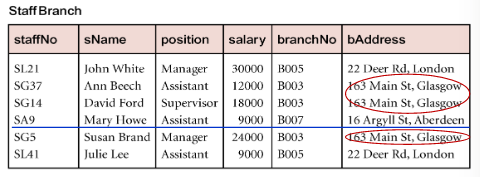
\includegraphics[scale=0.7]{anomalies}
\end{center}
\begin{itemize}
	\item Modification anomaly:
	\begin{itemize}
		\item we want to change the address of branch B003
		\item we must update it in many places (due to redundancy)
		\item problem: if we do not update one of them $\Rightarrow$ inconsistent data
	\end{itemize}
	\item Deletion anomaly:
	\begin{itemize}
		\item we want to delete staff with staffNo SA9 from the database
		\item this is the last staff member in branch B007
		\item Problem: we loose the details of this branch $\Rightarrow$ incomplete data
	\end{itemize}
	\item Insertion anomaly
	\begin{itemize}
		\item We want to add a new branch, which has no staff yet\\
	$\Rightarrow$ we must add Null into the attributes related to staff
		\item staffNo is aa private key $\Rightarrow$ violation of entity integrity
	\end{itemize}
\end{itemize}
\section{Functional data dependencies}
The fundamentals of normalization theory:
\begin{itemize}
	\item Functional data dependency:
	\begin{itemize}
		\item Let A and B be two sets of attributes; we say that
		\begin{center}
			"B is functionally dependent on A" (denoted $A\rightarrow B$)
		\end{center}
		if each value of A determines exactly one value of B
	\end{itemize}
	\item In a functional data dependency $(A\rightarrow B)$:
	\begin{itemize}
		\item determinant: the set of all attributes on the left hand side (i.e. A)
		\item dependent: the set of all attributes on the right hand side (i.e. B)
	\end{itemize}
	\item By the definition of relational keys:
	\begin{itemize}
		\item a candidate key is a minimal set of attributes, which functionally determine all attributes in a relation
		\item among all candidate keys, we choose (any) one of them to serve as the primary key
	\end{itemize}
\end{itemize}
\section{Functional dependencies}
\begin{itemize}
	\item \textbf{Full} functional dependency $A\rightarrow B$
	\begin{itemize}
		\item B is functionally dependent on A
		\item B is not functionally dependent on any proper subset of A
		\item Example: staffNo$\rightarrow$ sName
	\end{itemize}
	\item Partial functional dependency $A\rightarrow B$:
	\begin{itemize}
		\item B is functionally dependent on A
		\item B remains functionally dependent on at least one proper subset of A
		\item Example: staffNo,sName $\rightarrow$ branchNo
	\end{itemize}
	\item Transitive functional dependency:
	\begin{itemize}
		\item Functional dependencies $A\rightarrow B$ and $B\rightarrow C$
		\item Then the functional dependency $A\rightarrow C$ is called \textbf{transitive}
	\end{itemize}
\end{itemize}
\section{Normalization process}
\begin{itemize}
	\item Normalization is a multi-stage process
	\begin{itemize}
		\item The result of each stage is called a Normal form
		\item at each stage: check whether specific criteria are satisfied. If not: re-organise the data
	\end{itemize}
	\item We study the first 3 normal forms which are most important for practical applications
\end{itemize}
\begin{center}
	\includegraphics[scale=0.7]{"Normal Forms"}
\end{center}
\section{First Normal Form (1NF)}
\begin{itemize}
	\item Repeating group:
	\begin{itemize}
		\item an attribute (or group of attributes) that occurs with multiple values for a single occurence of the primary key
	\end{itemize}
	\item A table is in the un-normalised form (UNF):
	\begin{itemize}
		\item when it contains one or more repeating groups
		\item This does not conform with the definition of a relation
	\end{itemize}
	\item A table is in the First Normal Form (1NF) if it has:
	\begin{itemize}
		\item no repeating groups (every cell has one value)
		\item No identical rows
	\end{itemize}
\end{itemize}
How to bring a table into 1NF
\begin{itemize}
	\item One alternative would be:
	\begin{itemize}
		\item Repeat the appropriate columns horizontally
		\item Problem: a table must have a fixed number of columns
		\item We need a fixed (large) upper limit on the number of repetitions
		\item Many of these new columns would be empty $\Rightarrow$ waste of space
		\item Complicated querying: we need to search many columns to find the right item
	\end{itemize}
	\item Another alternative would be:
	\begin{itemize}
		\item For every multi valued attribute: one long string containing the whole list of items
		\item the same problems: long strings, difficult querying
	\end{itemize}
\end{itemize}
\begin{itemize}
	\item First method: one table solution
	\begin{itemize}
		\item enter appropriate data into the empty columns (by repeating data)
		\begin{center}
			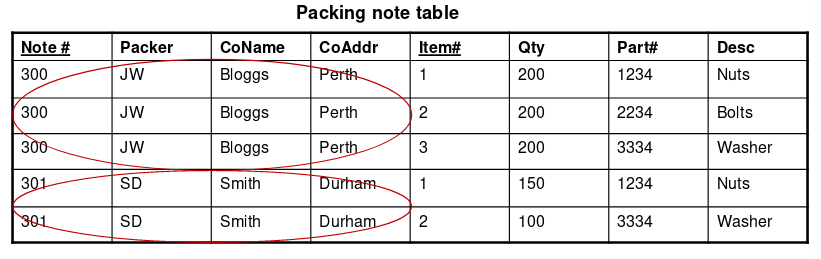
\includegraphics[scale=0.7]{1NF}
		\end{center}
		\item The resulting table is in 1NF, but still: we introduced a lot of redundancy (by repeating data)
	\end{itemize}
	\item Second method: two tables solution
	\begin{itemize}
		\item place the repeating data in a separate relation
		\item in the new relation place a copy of the original primary key
		\item this key now becomes a foreign key (to refer to the original relation)
		\item iterate until no repeated groups remain
	\end{itemize}
\begin{center}
	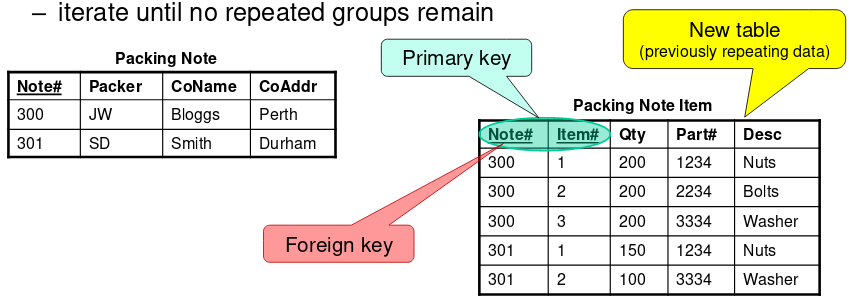
\includegraphics[scale=0.7]{1NF1}
\end{center}
	\item The resulting tables are in 1NF with much less redundancy than before
\end{itemize}
\section{Second normal form (2NF)}
\begin{itemize}
	\item A table is in the Second Normal Form (2NF) if:
	\begin{itemize}
		\item it is in 1NF and
		\item there are no partial functional dependencies i.e. every non key attribute is dependent on the whole primary key
	\end{itemize}
	\item Non-key attributes: all attributes that are not a part of the primary key
	\item 2NF applies to relations with composite keys
	\item When the primary key only has one attribute (single key) if the table is in 1NF $\Rightarrow$ it is also in 2NF
	\item How to bring a table into 2NF
	\begin{itemize}
		\item Remove the partially dependent attributes
		\item place them in a new relation, along with the copy of their determinant
	\end{itemize}
\end{itemize}
\end{document}